% Proposal (3.5p)
\section{Case Study: Notifications Manager}
\label{sec:notifications_manager}

\begin{figure*}[!htb]
 \centering
 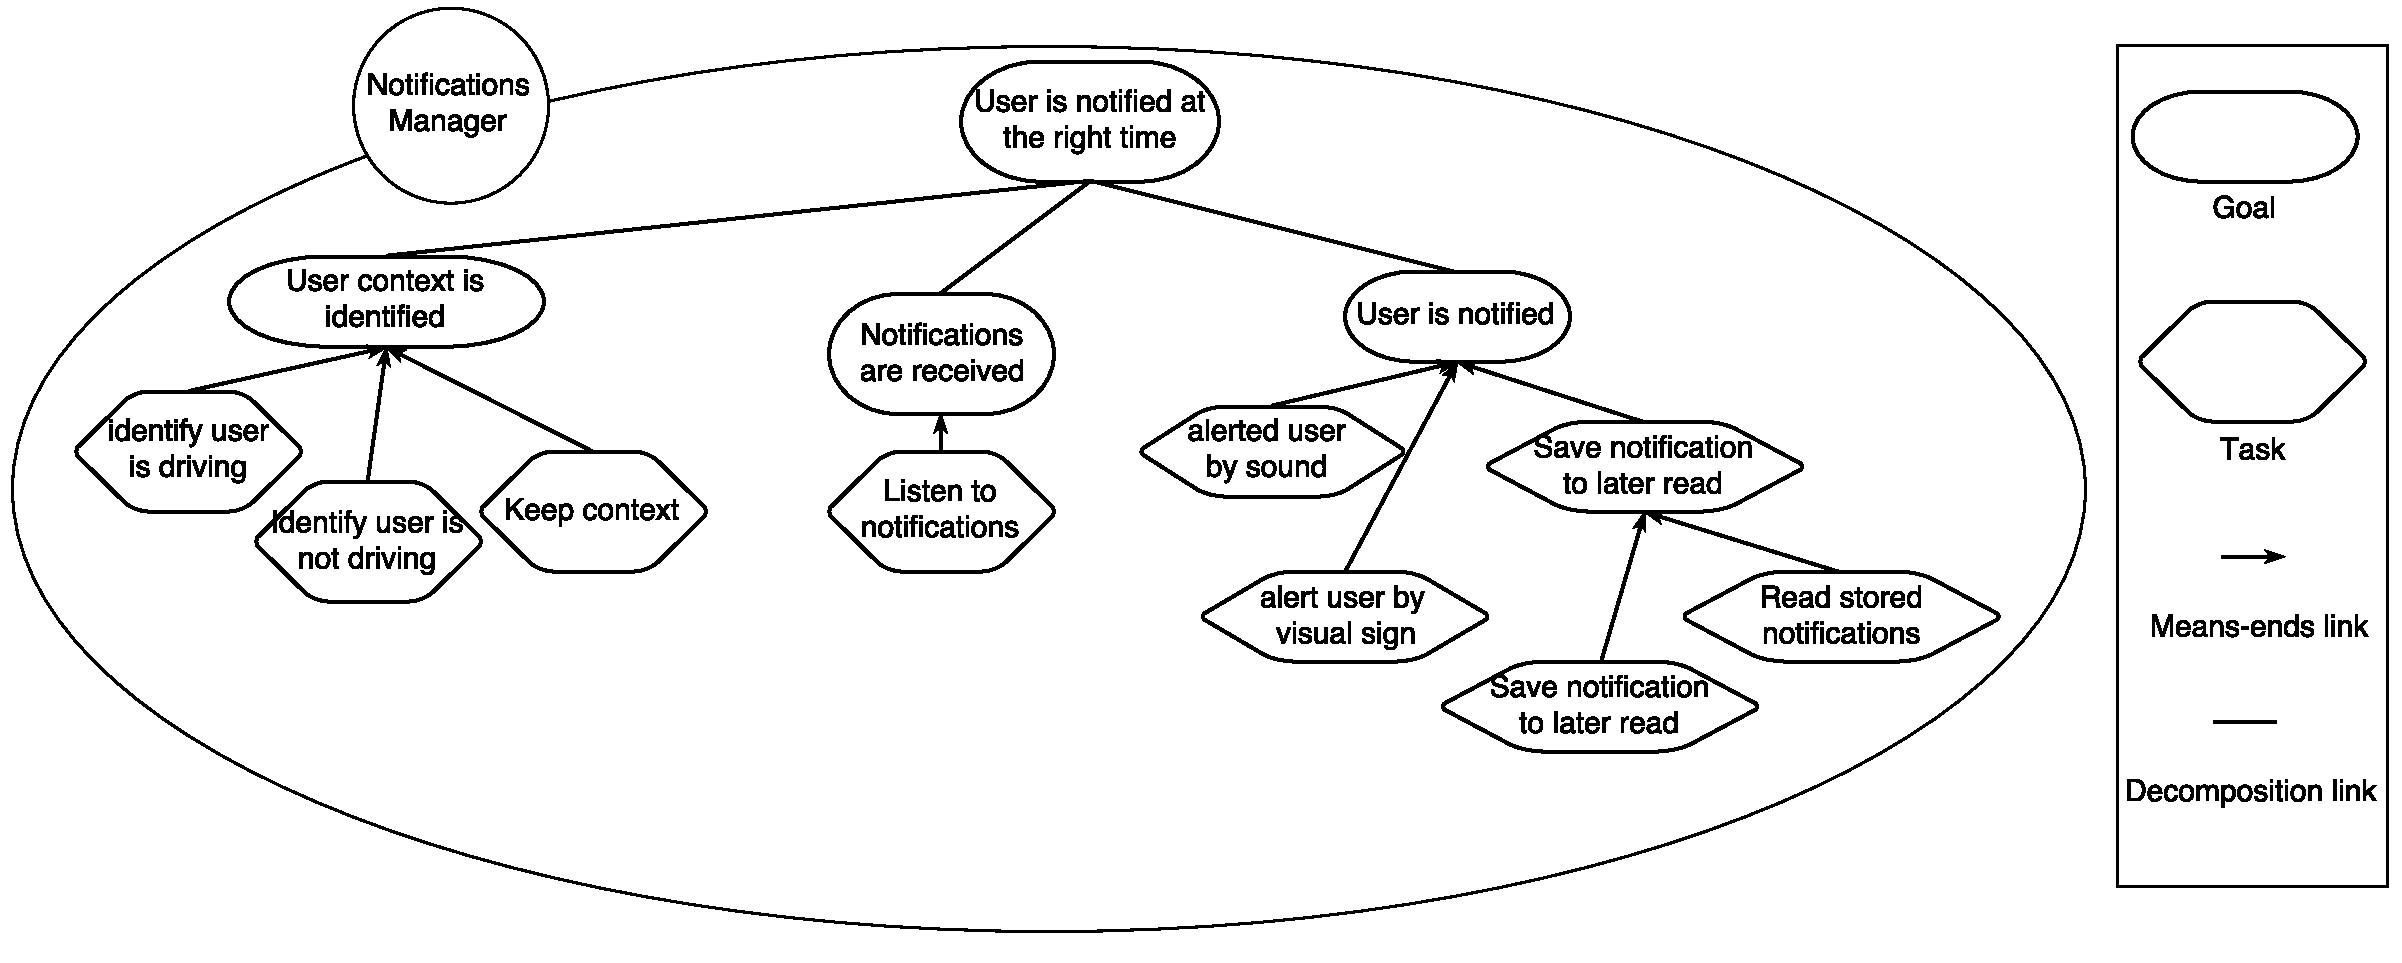
\includegraphics[width=\linewidth]{goal_model_notifications_manager}
 \caption{Tropos Goal model of the notifications manager}
\label{fig:goal_model_distraction_manager}
\end{figure*}

In this paper, we use a case study of a notifications manager application. The application is expected to assist a user access important information for a given context, while avoiding get distracted when she must focus on a demanding activity.

More specifically, here will present how this application should work on a car environment.
The system must identify a driving context, when notifications not related to driving must be avoided.
Other applications will request the user to be notified, but if the user will receive the notification instantly and the way it will receive the notification should depend on message type, urgency and the identified user context.
For example, imagine that a user is driving in a rain condition in a dangerous part of a road.
Some social network application tried to notify that the driver received a message. In this context, the user should not be notified in any way (indeed, even if it was a sunny day in a very secure road).
In the same situation, if the fuel is too low and the driver is passing by a gas station, the user should be notified instantly.

More generally, this application could be user in different environments. For example, in a Smart Home scenario, user that work at home could want that the many devices in her home network do not notify her if it is in working hours, if the notifications are not urgent or work related.

We identify two main challenges in developing such application for multiple environments: (1) available resources that can be used to sense the user context and to notify the user can vary a lot. (2) The application needs to be packaged and distributed differently for each device that it is supposed to run, it being a phone, a computer, a car, a watch, or an air conditioner. (3) Using current approaches, the user should manually install the application in each device it owns.
